\documentclass[11pt,dvipsnames]{article} % {{{

\usepackage{geometry}
\geometry{total={170mm,240mm}, left=20mm, top=20mm}

\usepackage[utf8]{inputenc}
\usepackage[spanish]{babel}
\usepackage{physics} 
\usepackage{siunitx} 
\usepackage{enumerate} 
\usepackage{pgfplots}
\usepackage{graphicx}
\usepackage{pgfplotstable}
\usepackage{tikz,pgfplots}
\usepackage{amsmath} 
\usepackage{xcolor}
\usepackage{float}
\usepackage{amsfonts}
\newcommand{\pce}{PCE}
\usepackage{dsfont}
%\usepackage{bbold}


\newcommand{\fref}[1]{fig.~\ref{#1}}  
\newcommand{\tref}[1]{table~\ref{#1}}
\newcommand{\Fref}[1]{Fig.~\ref{#1}}  
\newcommand{\Tref}[1]{Table~\ref{#1}}

\newcommand{\R}{\mathcal{R}}
\newcommand{\psii}{\psi_i}
\newcommand{\Pk}[1]{\ket{\psi_{#1} }}
\newcommand{\Pb}[1]{\bra{\psi_{#1} }}
\newcommand{\pk}{\ket{\psi}}
\newcommand{\M}{\mathcal{M}^{(N)}}
\newcommand{\E}{\mathcal{E}}
\newcommand{\Erho}{\mathcal{E}(\rho)}
\newcommand{\1}{\mathds{1}}
\newcommand{\ten}{\otimes}
\newcommand{\h}[1]{\colorbox{Yellow}{#1}}
\newcommand{\hi}{\mathcal{H}}
\newcommand{\txt}[1]{\text{#1}}
\newcommand{\here}{\h{\hspace{15cm}} }
\newcommand{\rhoi}{\dyad{\psii}{\psii}}
\newcommand{\ind}[2]{{{}^{#1}_{#2}}}
\newcommand{\rc}[1]{r_{#1}}
\newcommand{\pauli}[2]{\sigma_{#1}\otimes\sigma_{#2}}
\newcommand{\Er}{\E_{\mathcal{R}}}

%\usepackage[]{lineno}  \linenumbers
%\setlength\linenumbersep{3pt}
	

\usepackage{fancybox}
\usepackage{colortbl}
\usepackage{amsbsy}
\usepackage[draft,inline,nomargin]{fixme} \fxsetup{theme=color}
\FXRegisterAuthor{cp}{acp}{\color{blue}CP}
\FXRegisterAuthor{ja}{aja}{\color{RedViolet}JA}
\FXRegisterAuthor{dd}{ddg}{\color{red}DD}
% }}}
\begin{document}
% Titulo y otros {{{
\title{Mapeos PCE reducidos} 
%Title should be concise and to the point  
\author{J. A. de León}
\date{\today}  
\maketitle
% }}}

Sea $\E_{\mathcal{R}}$ un mapeo PCE de 2 qubits reducido, 
cuya acción es equivalente a 
\begin{align}
%\Er\qty(\rho^1_i)&=\Tr_j\qty[\E\qty(\rho^1_1\otimes\rho^1_2)], \\
\Er\qty(\rho_i)&=\Tr_j\qty[\E\qty(\stackrel{\sim}{\rho})], 
& i,j&=1,2; & i\neq j,
\label{•}
\end{align}
donde $\E$ es un mapeo PCE de 2 qubits, $\stackrel{\sim}{\rho}$ es
una matriz de densidad de 2 qubits y $\rho_i$ una matriz de densidad
de 1 qubit, con $i$ el qubit al que refiere.


Veamos a continuación en la representación de los tableros de 
los mapeos PCE un mapeo reducido $\Er$. La operación $\E$, 
representada por su tablero en la parte izquierda de las 2 figuras de 
abajo, no es una operación CP porque viola la regla de la potencia de 2 
componentes invariantes. Sin embargo, dos casos se presentan 
para las operaciones reducidas sobre cada uno de los qubits: (a) 
la operación sobre el primer 1 qubit es un canal PCE, y (b) la operación
reducida sobre el segundo qubit no es un canal cuántico porque 
no es CP, dado que viola la regla de la potencia de 2 para 1 qubit.
\begin{figure}[H]
    \centering
    \begin{minipage}{.4\textwidth}
        \centering
        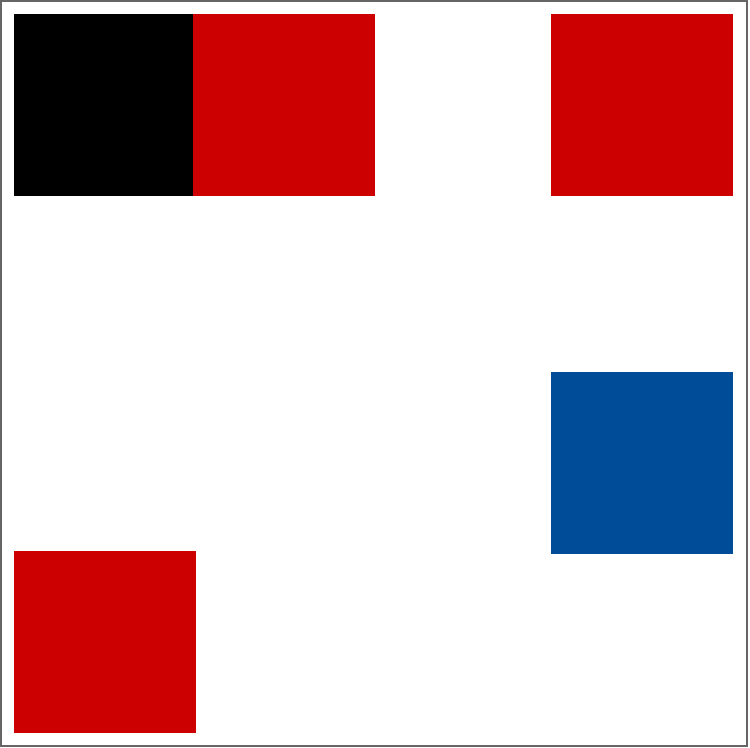
\includegraphics[height=4cm]{img/rndm-tab-2q-1}
    \end{minipage}
    $\stackrel{\Tr _2}{\longmapsto}$
    \begin{minipage}{0.4\textwidth}
        \centering
         
\includegraphics[height=4cm]{img/rndm-tab-1q1-1}
         \hfill
    \end{minipage}
\end{figure}

\begin{figure}[H]
    \centering
    \begin{minipage}{.4\textwidth}
        \centering
        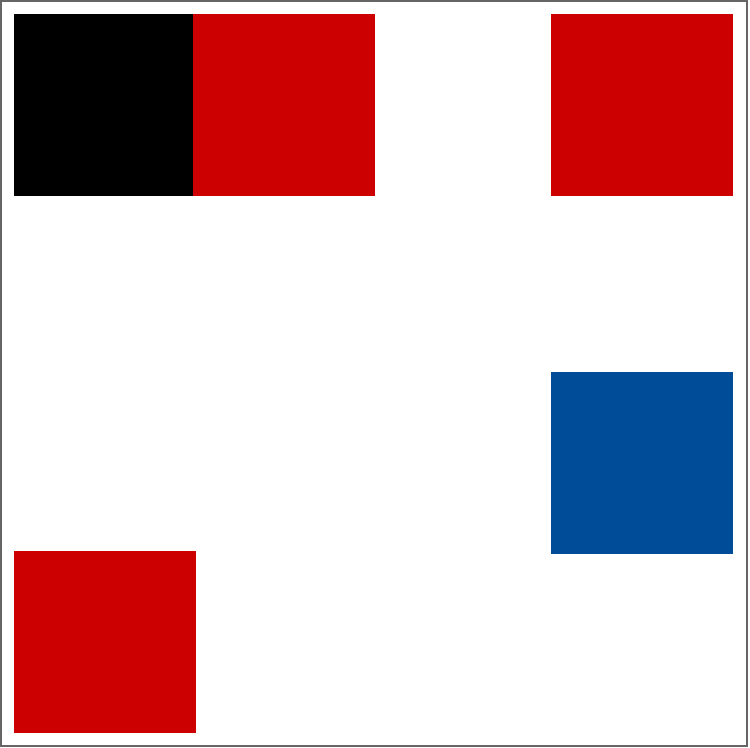
\includegraphics[height=4cm]{img/rndm-tab-2q-1}
    \end{minipage}
    $\stackrel{\Tr _1}{\longmapsto}$
    \begin{minipage}{0.4\textwidth}
        \centering
         
\includegraphics[height=4cm]{img/rndm-tab-1q2-1}
         \hfill
    \end{minipage}
\end{figure}

Otro mapeo PCE del que resultan las mismas operaciones reducidas
de 1 qubit es el siguiente:
\begin{figure}[H]
  \centering
  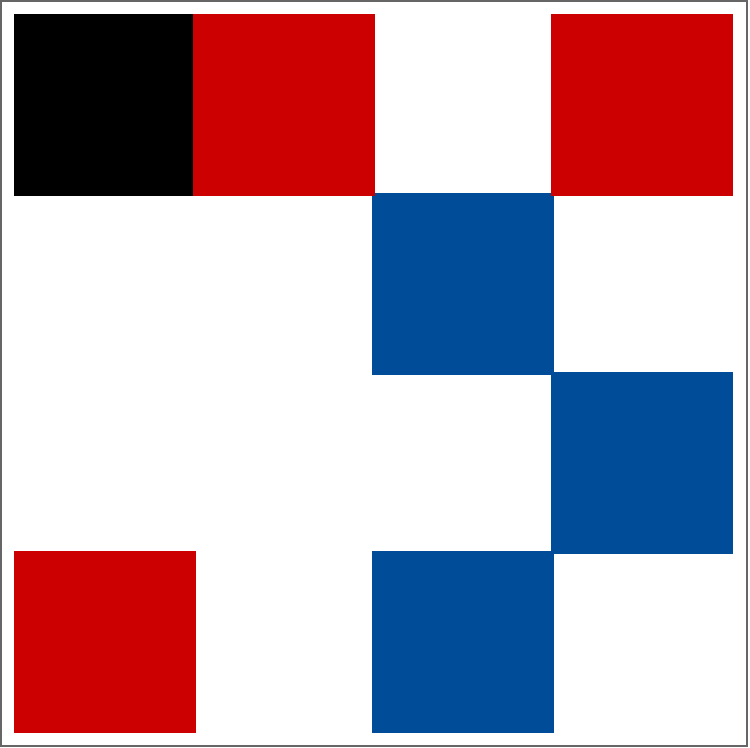
\includegraphics[height=4cm]{img/rndm-tab-2q-2}.
\end{figure}
Acabamos de presentar dos mapeos PCE de 2 qubits, cuyas 
operaciones reducidas de 1 qubit son iguales. Esto, con ayuda 
de la representación de los tableros, nos motiva a pensar que 
lo único necesario para entender las operaciones PCE reducidas 
es la acción de $\E$ sobre las componentes de la matriz de densidad
de 2 qubits, escrita como en \eqref{eq:dm-2q}, 
de la forma $r_{i0}$ y $r_{0j}$.

\begin{align}
\rho=\frac{1}{4}\sum _{i,j}r_{ij}\sigma_i\otimes\sigma_j
\label{eq:dm-2q}
\end{align}

Veamos a continuación una prueba analítica para la hipótesis que acabamos
de formular. Recordemos que un mapeo PCE de 2 qubits da como resultado
\begin{align}
\E (\rho)=\frac{1}{4}\sum _{i,j}r'_{ij}\sigma_i\otimes\sigma_j,
\label{eq:dm-2q}
\end{align}
con alguna cantidad $l$ de componentes $r'_{ij}=0$ y $(16-l)$
componentes que se mantienen invariantes $(r'_{ij}=r_{ij})$.
Luego, al calcular cualquiera de las dos operaciones reducidas
$\Er´$ da como resultado
\begin{align}
\Er (\rho_1)= \Tr_2\qty(\frac{1}{4}\sum _{i,j}r'_{ij}\sigma_i\otimes\sigma_j)
=
\frac{1}{2}\sum_ir'_{i0}\sigma_i,
\label{eq:er-1}
\end{align}
\begin{align}
\Er (\rho_2) = \Tr_1\qty(\frac{1}{4}\sum _{i,j}r'_{ij}\sigma_i\otimes\sigma_j)
=
\frac{1}{2}\sum_j r'_{0j}\sigma_j,
\label{eq:er-2}
\end{align}
por lo cual, para que \eqref{eq:er-1} y \eqref{eq:er-2} sean 
el resultado de un canal PCE de 1 qubit, el número de componentes 
que cumplen con $r'_{i0}=r_{i0}$ o $r'_{0j}$ debe ser una potencia 
de 2.

En conclusión, la condición para que un mapeo PCE de 2 qubits 
reducido sea un canal PCE de 1 qubit (CP) es independiente del estado del 
estado inicial del sistema total. Es decir, aunque el sistema total se encuentre
en un estado producto $(\rho_1\otimes\rho_2)$ o no la condición 
para que el mapeo reducido sea un canal PCE de 1 qubit es independiente
de la matriz de densidad inicial total y de cada matriz 
de densidad reducida (así se fijara cualquiera de los dos qubits).
La condición necesaria y suficiente para que un mapeo PCE 
de 2 qubits reducido sea un canal PCE de 1 qubit es que el número 
de componentes que el mapeo mantiene invariantes del conjunto 
$\{r_{i0}\}$ (o $\{r_{0j}\}$) obedezca la regla de $2^n$ $(1, 2$ o $4)$ 
componentes invariantes.

\bibliographystyle{unsrt}
\bibliography{references}
\vfill

\end{document}
